\documentclass[a4paper,14pt, unknownkeysallowed]{extreport}

\usepackage{cmap} % Улучшенный поиск русских слов в полученном pdf-файле
\usepackage[T2A]{fontenc} % Поддержка русских букв
\usepackage[utf8]{inputenc} % Кодировка utf8
\usepackage[english,russian]{babel} % Языки: русский, английский
\usepackage{enumitem}


\usepackage{threeparttable}

\usepackage[14pt]{extsizes}

\usepackage{caption}
\captionsetup{labelsep=endash}
\captionsetup[figure]{name={Рисунок}}

% \usepackage{ctable}
% \captionsetup[table]{justification=raggedleft,singlelinecheck=off}

\usepackage{amsmath}

\usepackage{geometry}
\geometry{left=30mm}
\geometry{right=10mm}
\geometry{top=20mm}
\geometry{bottom=20mm}

\usepackage{titlesec}
\titleformat{\section}
	{\normalsize\bfseries}
	{\thesection}
	{1em}{}
\titlespacing*{\chapter}{0pt}{-30pt}{8pt}
\titlespacing*{\section}{\parindent}{*4}{*4}
\titlespacing*{\subsection}{\parindent}{*4}{*4}

\usepackage{setspace}
\onehalfspacing % Полуторный интервал

\frenchspacing
\usepackage{indentfirst} % Красная строка

\usepackage{titlesec}
\titleformat{\chapter}{\LARGE\bfseries}{\thechapter}{20pt}{\LARGE\bfseries}
\titleformat{\section}{\Large\bfseries}{\thesection}{20pt}{\Large\bfseries}

\usepackage{multirow}
\usepackage{listings}
\usepackage{xcolor}

% Для листинга кода:
\lstset{%
	language=python,   					% выбор языка для подсветки	
	basicstyle=\small\sffamily,			% размер и начертание шрифта для подсветки кода
	numbers=left,						% где поставить нумерацию строк (слева\справа)
	numberstyle=\tiny,		     		% размер шрифта для номеров строк
	stepnumber=1,						% размер шага между двумя номерами строк
	numbersep=5pt,						% как далеко отстоят номера строк от подсвечиваемого кода
	frame=single,						% рисовать рамку вокруг кода
	tabsize=4,							% размер табуляции по умолчанию равен 4 пробелам
	captionpos=t,						% позиция заголовка вверху [t] или внизу [b]
	breaklines=true,					
	breakatwhitespace=true,				% переносить строки только если есть пробел
	backgroundcolor=\color{white},
	basicstyle=\footnotesize\ttfamily,
	keywordstyle=\color{blue},
	stringstyle=\color{red},
	commentstyle=\color{gray},
	showspaces=false,
    showstringspaces=false
}


\usepackage{pgfplots}
\usetikzlibrary{datavisualization}
\usetikzlibrary{datavisualization.formats.functions}


\lstset{
	literate=
	{а}{{\selectfont\char224}}1
	{б}{{\selectfont\char225}}1
	{в}{{\selectfont\char226}}1
	{г}{{\selectfont\char227}}1
	{д}{{\selectfont\char228}}1
	{е}{{\selectfont\char229}}1
	{ж}{{\selectfont\char230}}1
	{з}{{\selectfont\char231}}1
	{и}{{\selectfont\char232}}1
	{й}{{\selectfont\char233}}1
	{к}{{\selectfont\char234}}1
	{л}{{\selectfont\char235}}1
	{м}{{\selectfont\char236}}1
	{н}{{\selectfont\char237}}1
	{о}{{\selectfont\char238}}1
	{п}{{\selectfont\char239}}1
	{р}{{\selectfont\char240}}1
	{с}{{\selectfont\char241}}1
	{т}{{\selectfont\char242}}1
	{у}{{\selectfont\char243}}1
	{ф}{{\selectfont\char244}}1
	{х}{{\selectfont\char245}}1
	{ц}{{\selectfont\char246}}1
	{ч}{{\selectfont\char247}}1
	{ш}{{\selectfont\char248}}1
	{щ}{{\selectfont\char249}}1
	{ъ}{{\selectfont\char250}}1
	{ы}{{\selectfont\char251}}1
	{ь}{{\selectfont\char252}}1
	{э}{{\selectfont\char253}}1
	{ю}{{\selectfont\char254}}1
	{я}{{\selectfont\char255}}1
	{А}{{\selectfont\char192}}1
	{Б}{{\selectfont\char193}}1
	{В}{{\selectfont\char194}}1
	{Г}{{\selectfont\char195}}1
	{Д}{{\selectfont\char196}}1
	{Е}{{\selectfont\char197}}1
	{Ж}{{\selectfont\char198}}1
	{З}{{\selectfont\char199}}1
	{И}{{\selectfont\char200}}1
	{Й}{{\selectfont\char201}}1
	{К}{{\selectfont\char202}}1
	{Л}{{\selectfont\char203}}1
	{М}{{\selectfont\char204}}1
	{Н}{{\selectfont\char205}}1
	{О}{{\selectfont\char206}}1
	{П}{{\selectfont\char207}}1
	{Р}{{\selectfont\char208}}1
	{С}{{\selectfont\char209}}1
	{Т}{{\selectfont\char210}}1
	{У}{{\selectfont\char211}}1
	{Ф}{{\selectfont\char212}}1
	{Х}{{\selectfont\char213}}1
	{Ц}{{\selectfont\char214}}1
	{Ч}{{\selectfont\char215}}1
	{Ш}{{\selectfont\char216}}1
	{Щ}{{\selectfont\char217}}1
	{Ъ}{{\selectfont\char218}}1
	{Ы}{{\selectfont\char219}}1
	{Ь}{{\selectfont\char220}}1
	{Э}{{\selectfont\char221}}1
	{Ю}{{\selectfont\char222}}1
	{Я}{{\selectfont\char223}}1
}

\usepackage{graphicx}
\newcommand{\img}[3] {
	\begin{figure}[h!]
		\center{\includegraphics[height=#1]{img/#2}}
		\caption{#3}
		\label{img:#2}
	\end{figure}
}


\usepackage[justification=centering]{caption} % Настройка подписей float объектов

\usepackage[unicode,pdftex]{hyperref} % Ссылки в pdf
\hypersetup{hidelinks}

\usepackage{csvsimple}

\newcommand{\code}[1]{\texttt{#1}}

\usepackage{longtable}

\usepackage{array}
\usepackage{booktabs}
\usepackage{floatrow}

\floatsetup[longtable]{LTcapwidth=table}

% \def\UrlBreaks{\do\/\do-\do\_}

\makeatletter
\renewcommand*\l@chapter[2]{%
  \ifnum \c@tocdepth >\m@ne
    \addpenalty{-\@highpenalty}%
    \vskip 1.0em \@plus\p@
    \setlength\@tempdima{1.5em}%
    \begingroup
      \parindent \z@ \rightskip \@pnumwidth
      \parfillskip -\@pnumwidth
      \leavevmode \bfseries
      \advance\leftskip\@tempdima
      \hskip -\leftskip
      #1\nobreak\normalfont\leaders\hbox{$\m@th
        \mkern \@dotsep mu\hbox{.}\mkern \@dotsep
        mu$}\hfill\nobreak\hb@xt@\@pnumwidth{\hss #2}\par
      \penalty\@highpenalty
    \endgroup
  \fi}
\makeatother

\begin{document}



\begin{titlepage}
	\newgeometry{pdftex, left=2cm, right=2cm, top=2.5cm, bottom=2.5cm}
	\fontsize{12pt}{12pt}\selectfont
	\noindent \begin{minipage}{0.15\textwidth}
		
\includegraphics[width=\linewidth]{img/b_logo.jpg}
	\end{minipage}
	\noindent\begin{minipage}{0.9\textwidth}\centering
		\textbf{Министерство науки и высшего образования Российской Федерации}\\
		\textbf{Федеральное государственное бюджетное образовательное учреждение высшего образования}\\
		\textbf{«Московский государственный технический университет имени Н. Э.~Баумана}\\
		\textbf{(национальный исследовательский университет)»}\\
		\textbf{(МГТУ им. Н. Э.~Баумана)}
	\end{minipage}
	
	\noindent\rule{18cm}{3pt}
	\newline\newline
	\noindent ФАКУЛЬТЕТ $\underline{\text{«Информатика и системы управления»~~~~~~~~~~~~~~~~~~~~~~~~~~~~~~~~~~~~~~~~~~~~~~~~~~~~~~~}}$ \newline\newline
	\noindent КАФЕДРА $\underline{\text{«Программное обеспечение ЭВМ и информационные технологии»~~~~~~~~~~~~~~~~~~~~~~~}}$\newline\newline\newline\newline\newline\newline
	
	
	\begin{center}
		\noindent\begin{minipage}{1.3\textwidth}\centering
		\Large\textbf{Отчёт по лабораторной работе №1}\newline
		\textbf{по курсу "Моделирование"}\newline\newline\newline\newline\newline
		\end{minipage}
	\end{center}
	
	\noindent\textbf{Тема} 			$\underline{\text{Решение задачи Коши методами Пикара, Эйлера и Рунге-Кутта}}$\newline\newline
	\noindent\textbf{Студент} 		$\underline{\text{Ковалец К. Э.}}$\newline\newline
	\noindent\textbf{Группа} 		$\underline{\text{ИУ7-63Б}}$\newline\newline
	\noindent\textbf{Преподаватель} $\underline{\text{Градов В. М.}}$\newline
	
	\begin{center}
		\vfill
		Москва~---~\the\year
		~г.
	\end{center}
	\restoregeometry
\end{titlepage}



\setcounter{page}{2}

\chapter{Задание}

\section{Тема работы}

Программная реализация приближенного аналитического метода и численных алгоритмов первого и второго порядков точности при решении задачи Коши для ОДУ.

\section{Цель работы}

Получение навыков решения задачи Коши для ОДУ методами Пикара и явными методами первого порядка точности (Эйлера) и второго порядка точности (Рунге-Кутта).

\section{Исходные данные}

ОДУ, не имеющее аналитического решения

\begin{equation}
	{\begin{cases}
			u'(x) = x^2 + u^2 \\
			u(0) = 0
		\end{cases}}
		\label{eq:ref0}
\end{equation}

\section{Результат работы программы}

\begin{itemize}
	\item Таблица, содержащая значения аргумента с заданным шагом в интервале $[0, x_{max}]$ и результаты расчета функции $u(x)$ в приближениях Пикара (от 1-го до 4-го), а также
	численными методами. Границу интервала $x_{max}$ выбирать максимально возможной из условия, чтобы численные методы обеспечивали точность вычисления решения уравнения
	$u(x)$ до второго знака после запятой.
	\item График функции в диапазоне [$-x_{max}$,  $x_{max}$].
\end{itemize}



\chapter{Теоретические сведение}

Имеем ОДУ, у которого отсутствует аналитическое решение:

\begin{equation}
	{\begin{cases}
			u'(x) = f(x,u) \\
			u(\xi) = \eta
		\end{cases}}
		\label{eq:ref1}
\end{equation}

Для решения данного ОДУ были использованы 3 алгоритма.

\section{Метод Пикара}

Имеем:

\begin{equation}
    \label{solution}
    u(x) = \eta +  \int_{\xi}^{x} f(t,u(t)) \,dt
\end{equation}

Строим ряд функций:

\begin{equation}
    \label{sol}
    y^{(s)} = \eta +  \int_{\xi}^{x} f(t,y^{(s-1)}(t)) \,dt, \quad \quad
    y^{(0)} = \eta
\end{equation}

Построим 4 приближения для уравнения (\ref{solution}):

\begin{equation}
    \label{f1}
    y^{(1)}(x) = 0 + \int_{0}^{x} t^2 \,dt = \frac{x^3}{3}
\end{equation}

\begin{equation}
    \label{f2}
    y^{(2)}(x) = 0 + \int_{0}^{x} (t^2 + \left(\frac{t^3}{3}\right)^2) \,dt = \frac{x^3}{3} + \frac{x^7}{63}
\end{equation}

\begin{equation}
    \label{f3}
    y^{(3)}(x) = 0 + \int_{0}^{x} (t^2 + \left(\frac{t^3}{3} + \frac{t^7}{63}\right)^2) \,dt = \frac{x^3}{3} + \frac{x^7}{63} + \frac{2x^{11}}{2079} + \frac{x^{15}}{59535}
\end{equation}

\begin{equation}
    \begin{split}
        \label{f4}
        y^{(4)}(x) = 0 + \int_{0}^{x} (t^2 + \left(\frac{t^3}{3} + \frac{t^7}{63} + \frac{2t^{11}}{2079} + \frac{t^{15}}{59535}\right)^2) \,dt = \frac{x^3}{3} + \frac{x^7}{63} + \frac{2x^{11}}{2079} +\\
        \frac{13x^{15}}{218295} + \frac{82x^{19}}{37328445} + \frac{662x^{23}}{10438212015} + \frac{4x^{27}}{3341878155} + \frac{x^{31}}{109876903975}
    \end{split}
\end{equation}


\section{Метод Эйлера}

\begin{equation}
    \label{ey}
    y^{(n+1)}(x) = y^{(n)}(x) + h \cdot f(x_{n}, y^{(n)})
\end{equation}

\indent Порядок точности: $O(h)$.


\section{Метод Рунге-Кутта}

\begin{equation}
    \label{rk}
    y^{n+1}(x) = y^{n}(x) + h ((1-\alpha) R_1 + \alpha R_2)
\end{equation}\newline

где $R1 = f(x_{n}, y^{n})$, $R2 = f(x_{n} + \frac{h}{2\alpha}, y^{n} + \frac{h}{2\alpha}R_1)$, $\alpha = \frac{1}{2}$ или 1\newline

Порядок точности: $O(h^2)$.

\chapter{Исходный код алгоритмов}

\begin{center}
\captionsetup{justification=raggedright,singlelinecheck=off}
\begin{lstlisting}[label=lst:parallel_processing,caption=Исходный код алгоритмов]
import matplotlib.pyplot as plt
from color import * 


MAX_X = 1
STEP  = 1e-4


def f(x, y):
	return pow(x, 2) + pow(y, 2)


def PicarApprox1(x):
	return pow(x, 3) / 3


def PicarApprox2(x):
	return PicarApprox1(x) + \
		pow(x, 7) / 63
		

def PicarApprox3(x):
	return PicarApprox2(x)    + \
		2 * pow(x, 11) / 2079 + \
			pow(x, 15) / 59535


def PicarApprox4(x):
	return PicarApprox2(x)             + \
		2   * pow(x, 11) / 2079        + \
		13  * pow(x, 15) / 218295      + \
		82  * pow(x, 19) / 37328445    + \
		662 * pow(x, 23) / 10438212015 + \
		4   * pow(x, 27) / 3341878155  + \
				pow(x, 31) / 109876903975


def Picar(x_max, h, PicarApprox):
	result = []
	x, y = 0, 0

	while abs(x) < abs(x_max):
		result.append(y)
		x += h
		y = PicarApprox(x)
	
	return result


def Euler(x_max, h):
	result = []
	x, y = 0, 0
	
	while abs(x) < abs(x_max):
		result.append(y)
		y = y + h * f(x, y)
		x += h

	return result


def RungeKutta(x_max, h):
	result = []
	coeff = h / 2
	x, y = 0, 0
	
	while abs(x) < abs(x_max):
		result.append(y)
		y = y + h * f(x + coeff, y + coeff * f(x, y))
		x += h
	
	return result


def generate_x(x_max, step):
	result = []
	x = 0

	while abs(x) < abs(x_max):
		result.append(round(x, 3))
		x += step

	return result


def print_res_table(x_arr, picar_approx1_arr, picar_approx2_arr, 
					picar_approx3_arr, picar_approx4_arr, 
					euler_arr, runge_kutta):

	print("\n%s  X   | PicarApprox1 | PicarApprox2 | PicarApprox3 | PicarApprox4 |     Euler    | RungeKutta \n" 
				"-------------------------------------------------- ---------------------------------------------%s"
	%(PURPLE, BASE))


	for i in range(len(x_arr)):
		if i % 500 == 0:
			print("%5.2f %s|%s%12.5f  %s|%s%12.5f  %s|%s%12.5f  %s|%s%12.5f  %s|%s%12.5f  %s|%s%12.5f  " \
			%(x_arr[i],             PURPLE, BASE, 
				picar_approx1_arr[i], PURPLE, BASE,
				picar_approx2_arr[i], PURPLE, BASE,
				picar_approx3_arr[i], PURPLE, BASE,
				picar_approx4_arr[i], PURPLE, BASE,
				euler_arr[i],         PURPLE, BASE,
				runge_kutta[i]
			))

	print()


def build_graph(x_arr, picar_approx1_arr, picar_approx2_arr, 
				picar_approx3_arr, picar_approx4_arr, 
				euler_arr, runge_kutta):

	fig1 = plt.figure(figsize = (10, 7))
	plot = fig1.add_subplot()
	plot.plot(x_arr, picar_approx1_arr,  label = "PicarApprox1")
	plot.plot(x_arr, picar_approx2_arr,  label = "PicarApprox2")
	plot.plot(x_arr, picar_approx3_arr,  label = "PicarApprox3")
	plot.plot(x_arr, picar_approx4_arr,  label = "PicarApprox4")
	plot.plot(x_arr, euler_arr,          label = "Euler")
	plot.plot(x_arr, runge_kutta,        label = "RungeKutta")

	plt.legend()
	plt.grid()
	plt.title("Сравнение алгоритмом")

	plt.show()


def main():

	x_arr			  = generate_x(MAX_X, STEP)
	picar_approx1_arr = Picar(MAX_X, STEP, PicarApprox1)
	picar_approx2_arr = Picar(MAX_X, STEP, PicarApprox2)
	picar_approx3_arr = Picar(MAX_X, STEP, PicarApprox3)
	picar_approx4_arr = Picar(MAX_X, STEP, PicarApprox4)
	euler_arr 		  = Euler(MAX_X, STEP)
	runge_kutta 	  = RungeKutta(MAX_X, STEP)

	print_res_table(x_arr, picar_approx1_arr, picar_approx2_arr, 
					picar_approx3_arr, picar_approx4_arr, 
					euler_arr, runge_kutta)

	x_arr = generate_x(-MAX_X, -STEP)
	x_arr.reverse()
	x_arr.extend(generate_x(MAX_X, STEP))

	picar_approx1_arr = Picar(-MAX_X, -STEP, PicarApprox1)
	picar_approx1_arr.reverse()
	picar_approx1_arr.extend(Picar(MAX_X, STEP, PicarApprox1))

	picar_approx2_arr = Picar(-MAX_X, -STEP, PicarApprox2)
	picar_approx2_arr.reverse()
	picar_approx2_arr.extend(Picar(MAX_X, STEP, PicarApprox2))

	picar_approx3_arr = Picar(-MAX_X, -STEP, PicarApprox3)
	picar_approx3_arr.reverse()
	picar_approx3_arr.extend(Picar(MAX_X, STEP, PicarApprox3))

	picar_approx4_arr = Picar(-MAX_X, -STEP, PicarApprox4)
	picar_approx4_arr.reverse()
	picar_approx4_arr.extend(Picar(MAX_X, STEP, PicarApprox4))

	euler_arr = Euler(-MAX_X, -STEP)
	euler_arr.reverse()
	euler_arr.extend(Euler(MAX_X, STEP))

	runge_kutta = RungeKutta(-MAX_X, -STEP)
	runge_kutta.reverse()
	runge_kutta.extend(RungeKutta(MAX_X, STEP))

	build_graph(x_arr, picar_approx1_arr, picar_approx2_arr, 
				picar_approx3_arr, picar_approx4_arr, 
				euler_arr, runge_kutta)


if __name__ == "__main__":
	main()

\end{lstlisting}
\end{center}


\chapter{Результаты работы программы}

\begin{figure}[h]
	\centering
	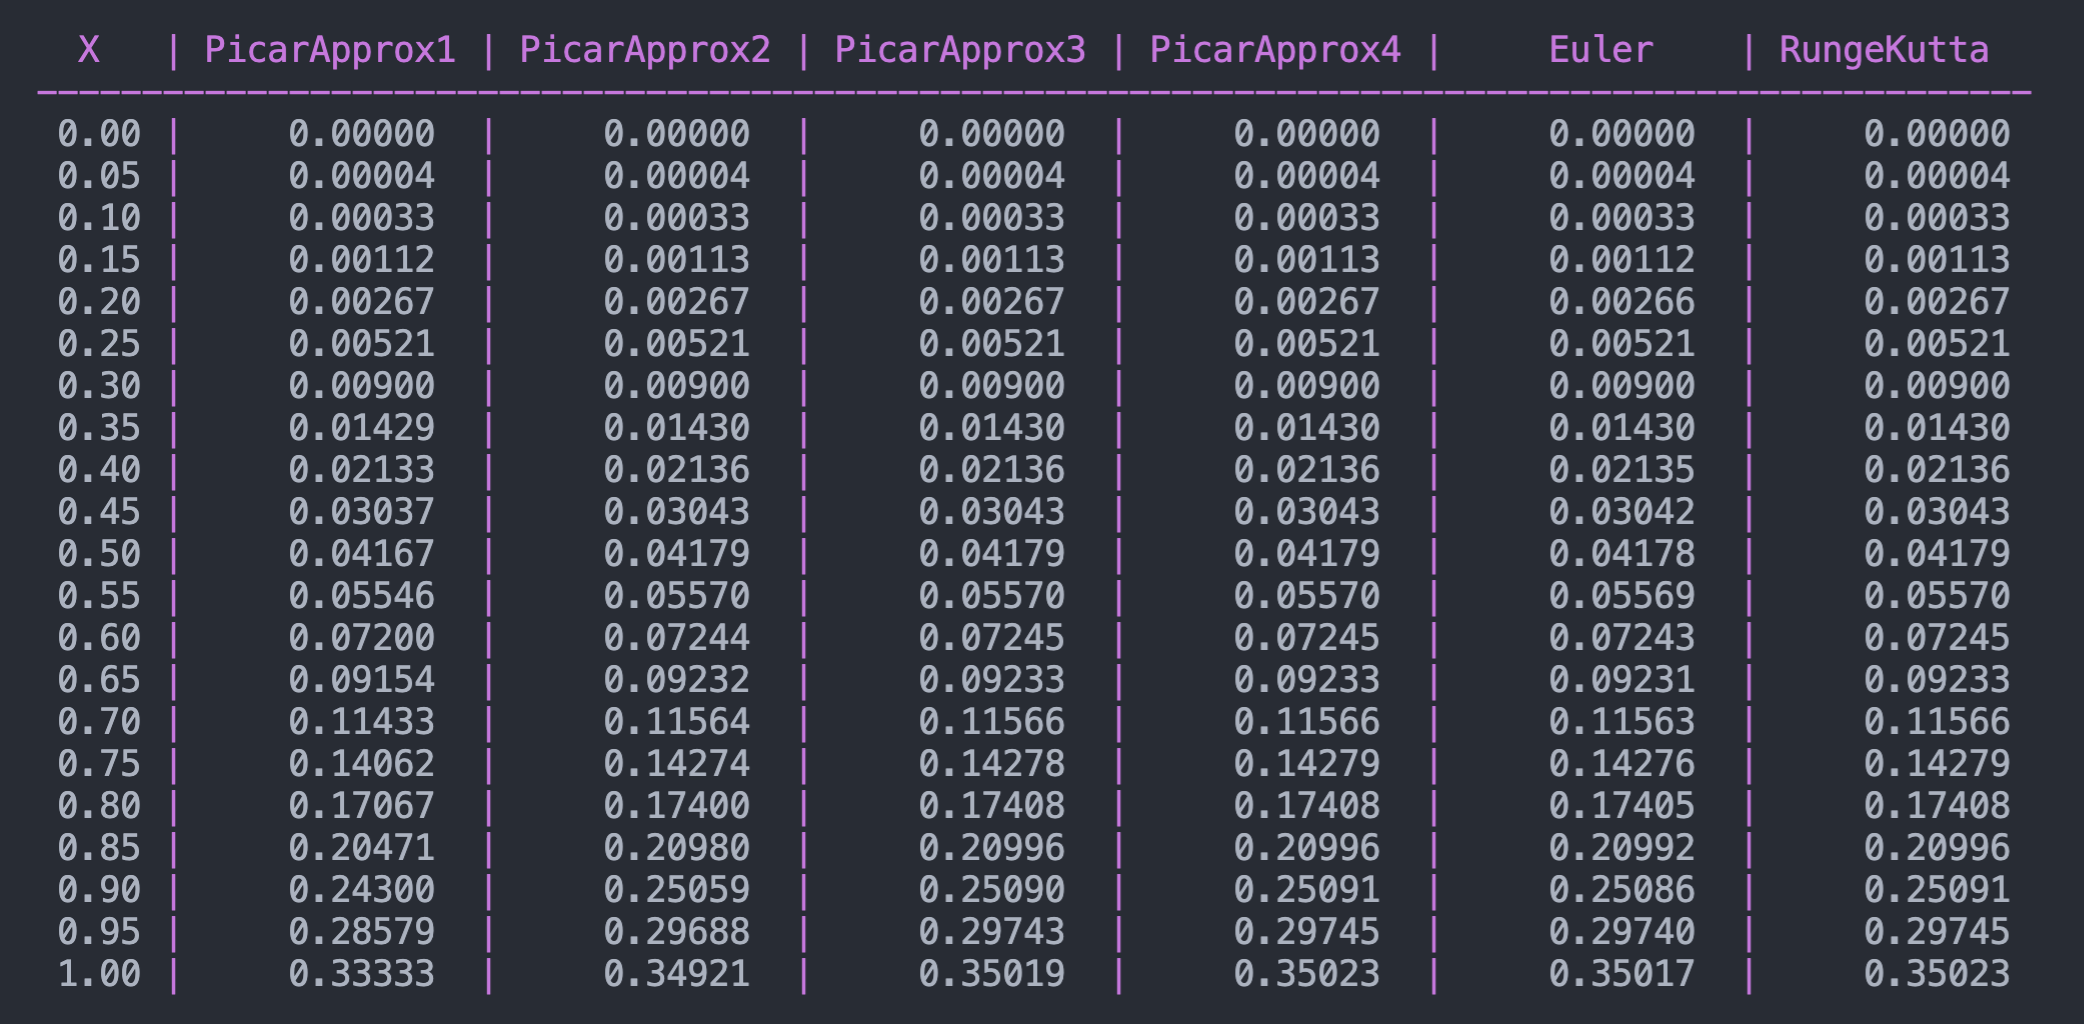
\includegraphics[scale=0.45]{img/table.png}
	\caption{Демонстрация работы программы}
	\label{fig:table}
\end{figure}

\begin{figure}[h]
	\centering
	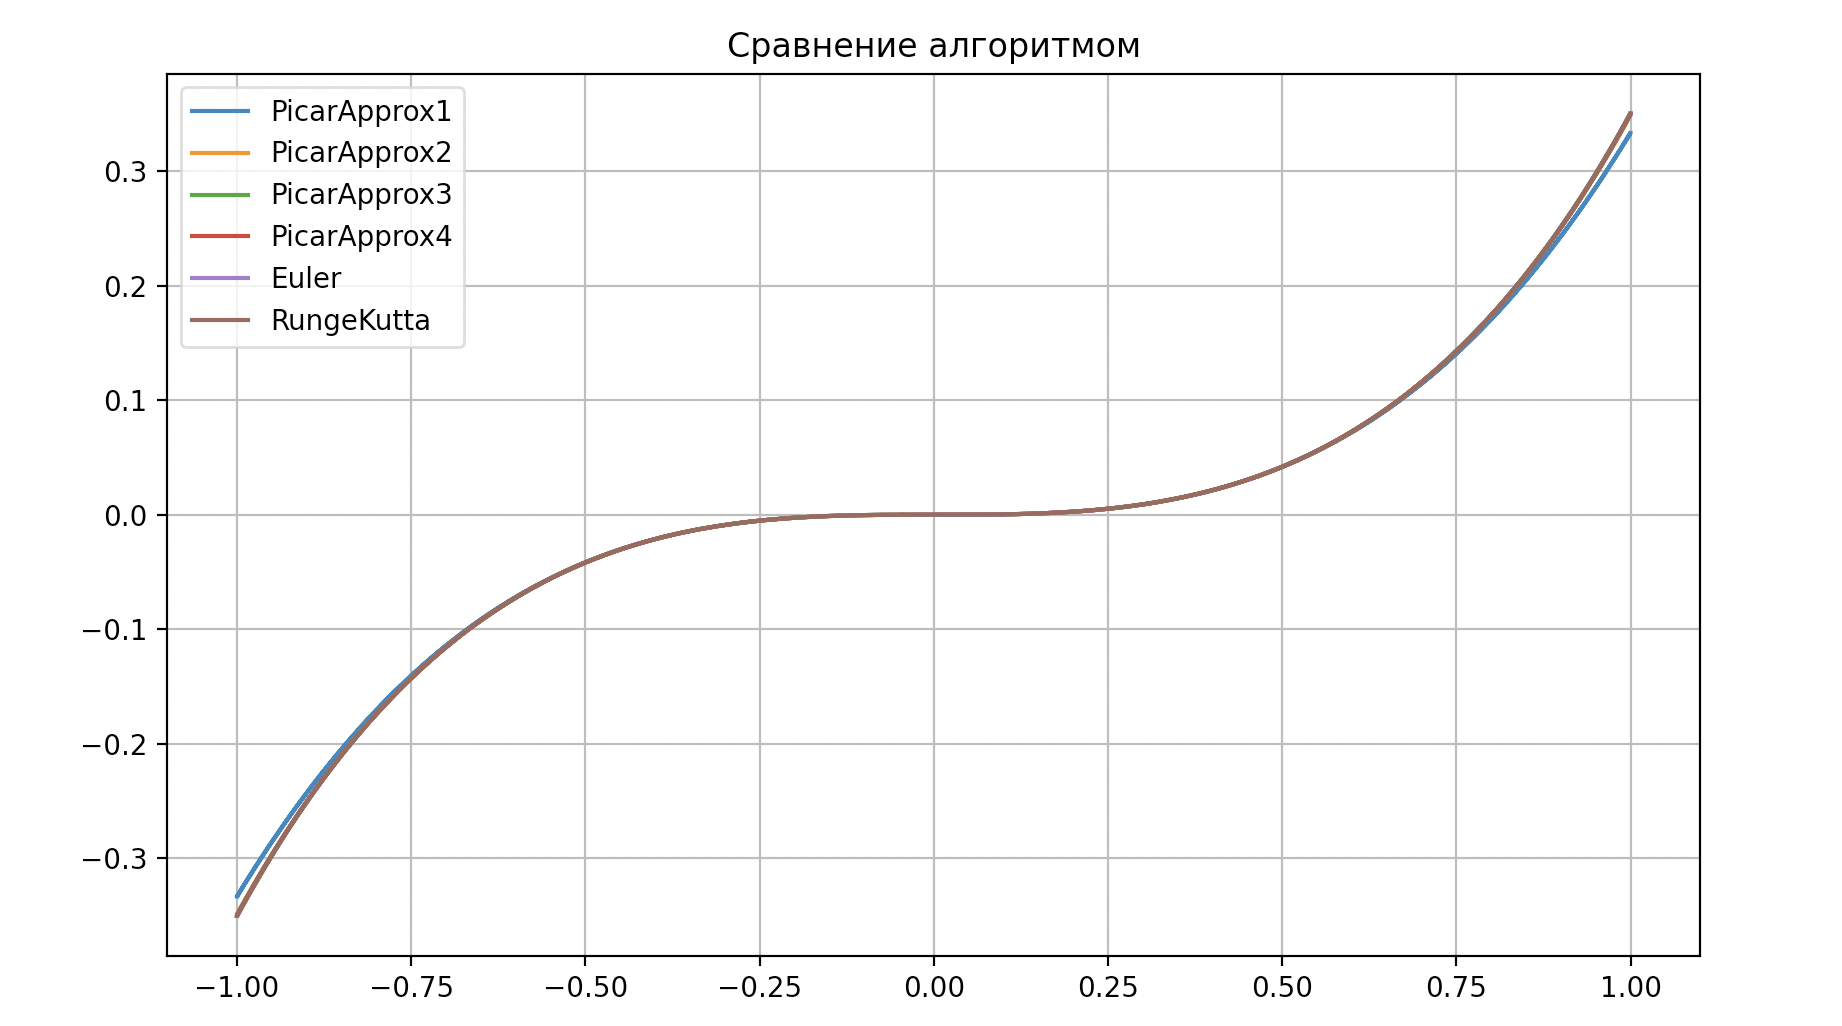
\includegraphics[scale=0.49]{img/graph.png}
	\caption{График функции}
	\label{fig:graph}
\end{figure}

\chapter{Ответы на контрольные вопросы}

\section{Вопрос 1}

\subsection{Задание}
Укажите интервалы значений аргумента, в которых можно считать решением заданного уравнения каждое из первых 4-х приближений Пикара, т.е. для каждого приближения указать свои границы применимости. Точность результата оценивать до второй цифры после запятой. Объяснить свой ответ.

\subsection{Ответ}
Для того, чтобы указать интервалы значений аргумента, в которых можно считать решением заданного уравнения каждое из первых 4-х приближений проанализируем полученные значения. Так как нам дано начальное приближение, то левой границей будет 0. Для определения правой границы границы мы будем анализировать полученные решения методом Пикара для конкретного приближения и сравнивать со значениями более высоких порядков приближения и с результатами численных методов при определенном шаге.

\begin{itemize}
	\item Для 1-го приближения искомым интервалом будет [0, 0.89].
	\item Для 2-го приближения искомым интервалом будет [0, 1.12].
	\item Для 3-го приближения искомым интервалом будет [0, 1.34].
	\item Для 4-го приближения искомым интервалом будет [0, 1.4].
\end{itemize}

\section{Вопрос 2}

\subsection{Задание}
Пояснить, каким образом можно доказать правильность полученного результата при фиксированном значении аргумента в численных методах.

\subsection{Ответ}
В численных методах правильность полученного результата, при фикси­ рованном значении аргумента, доказывается путем уменьшения шага. Правильно полученный результат -- это когда при уменьшение шага значение аргумента незна­ чительно (или вообще) не меняется.

\section{Вопрос 3}

\subsection{Задание}
Каково значение решения уравнения в точке x = 2, т.е. привести значение u(2).

\subsection{Ответ}
Примерно 317.490

\section{Вопрос 4}

\subsection{Задание}
Дайте оценку точки разрыва решения уравнения.

\section{Вопрос 5}

\subsection{Задание}
Покажите, что метод Пикара сходится к точному аналитическому решению уравнения

\begin{equation}
	{\begin{cases}
			u'(x) = x^2 + u \\
			u(0) = 0
		\end{cases}}
\end{equation}

\end{document}
